\documentclass{article}%
\usepackage[T1]{fontenc}%
\usepackage[utf8]{inputenc}%
\usepackage{lmodern}%
\usepackage{textcomp}%
\usepackage{lastpage}%
\usepackage[head=40pt,margin=0.5in,bottom=0.6in]{geometry}%
\usepackage{graphicx}%
%
\title{\textbf{Trabajadores públicos reclamaron por sus derechos laborales}}%
\author{YOSELIN GONZÁLEZ}%
\date{06/10/2018}%
%
\begin{document}%
\normalsize%
\maketitle%
\textbf{URL: }%
http://www.eluniversal.com/politica/22487/trabajadores{-}publicos{-}reclamaron{-}por{-}sus{-}derechos{-}laborales\newline%
%
\textbf{Periodico: }%
EU, %
ID: %
22487, %
Seccion: %
politica\newline%
%
\textbf{Palabras Claves: }%
NO\_TIENE\newline%
%
\textbf{Derecho: }%
2.3, %
Otros Derechos: %
, %
Sub Derechos: %
2.3.4\newline%
%
\textbf{EP: }%
SI\newline%
\newline%
%
\textbf{\textit{Se concentraron en 20 estados del país en las diferentes inspectorías del trabajo, para exigir mejorías en los salarios y que se respeten los contratos colectivos}}%
\newline%
\newline%
%
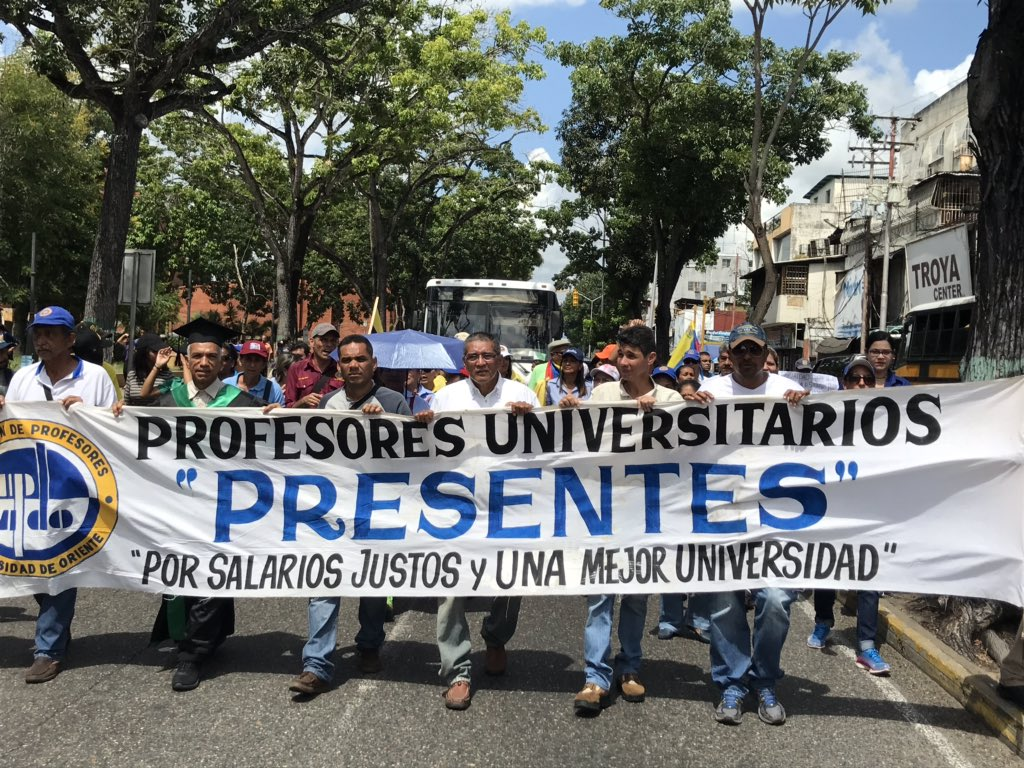
\includegraphics[width=300px]{43.jpg}%
\newline%
%
Docentes, trabajadores del área de salud y de educación, estudiantes, jubilados, pensionados, sociedad civil y sindicatos, se concentraron en la Plaza Caracas, a las afueras del Ministerio del Trabajo para exigir respeto a los derechos laborales, contratos colectivos y mejoras salariales.%
\newline%
%
La concentración fue convocada por el Frente Amplio, con el fin de hacer la entrega de un documento, que es el acuerdo alcanzado en la pasada asamblea de gremios y sindicatos, que exige el reintegro de los derechos laborales, méritos y beneficios logrados tras años de luchas reivindicativas.%
\newline%
%
Este escrito que fue recibido por el Presidente del Sindicato del Ministerio del Trabajo, y estaba dirigido al ministro Eduardo Piñate, quien no atendió~a los trabajadores.%
\newline%
%
Por otra parte, Ana Rosario Contreras,  presidenta del Colegio de Enfermeras del Distrito Capital, exigió al ejecutivo  “respetar al artículo 91 de la Constitución” al mencionar que el “Gobierno debe garantizar un salario mínimo para que podamos tener calidad de vida y no estar en pobreza extrema, como es la cruda realidad de los venezolanos”.%
\newline%
%
La protesta se extendió a 20 estados del país, entre ellos: Aragua, Guárico, Miranda, Táchira, Anzoátegui, Apure, Portuguesa, Zulia entre otros.%
\newline%
%
Los trabajadores reclaman por el cumplimiento de las convenciones colectivas, las cuales se han visto afectadas, negadas o eliminadas tras la decisión gubernamental de imponer un tabulador salarial con base al salario mínimo, desde septiembre, actualmente calculado en 1.800 bolívares soberanos.%
\newline%
%
En Monagas%
\newline%
%
En el estado oriental participaron los empleados y trabajadores de educación superior, como el Pedagógico de Maturín y la Universidad de Oriente, UDO, cuyos docentes se han visto afectados por el tema salarial, se mostraron muy  preocupados por la migración de docentes y estudiantes.%
\newline%
%
En Nueva Esparta%
\newline%
%
La comisión designada no pudo entregar el documento, por la falta de alguna autoridad que lo recibiera, además la inspectoría se negó a cualquier posibilidad de diálogo. La próxima entrega está prevista hacerla ante la delegación regional de la Defensoría del Pueblo, informó la corresponsal de El Universal.%
\newline%
%
Denuncias por Twitter%
\newline%
%
Mediante diferentes tuits y fotografías se evidencian a funcionarios de Poli{-}Guárico y Poli{-}Roscio fotografiando a representantes gremiales que se encontraban en la manifestación.%
\newline%
%
Asimismo, en Maracay estado Aragua, un piquete de la Policía Nacional impidió el paso de la marcha; sin embargo se designó una comisión de siete representantes de los sectores para que entregara el documento en la Inspectoría del Trabajo.%
\newline%
%
En Barquisimeto, médicos y enfermeras se preguntan ¿Dónde están los reales para la salud?%
\newline%
%
Antecedentes~a la protesta%
\newline%
%
Según estudios del Observatorio Venezolano de Conflictividad Social (OVCS), en agosto pasado se registraron 894 manifestaciones de diversa índole, lo que equivale a un promedio de 30 protestas diarias. Lo que registró un aumento del 20\% respecto a agosto 2017 (742 protestas).%
\newline%
%
El sondeo realizado, arroja que  en Caracas, Miranda, Bolívar, Mérida, Táchira y Zulia,  se alcanzó el mayor número de eventos por marchas y cierres de calles.%
\newline%
%
Aseguraron que agosto, coincidió con la entrada en vigor del proceso de reconversión monetaria impulsado por Maduro; por lo que el 88\% de las protestas estuvieron relacionadas con el rechazo a las medidas económicas anunciadas por el gobierno; exigencias laborales del sector de la salud, de los estudiantes y transportistas; demandas por derechos sociales y otras originadas por el colapso de servicios básicos como electricidad, agua potable y gas.%
\newline%
%
Más de las 347 protestas,  estuvieron relacionadas con problemas salariales y de contratos colectivos, destacan.%
\newline%
%
\end{document}